\documentclass[letterpaper,10pt]{article}

\usepackage{enumitem}
\usepackage{titling}
\usepackage{listings,listings-rust}
\usepackage{url}
\usepackage{soul}
\usepackage{hyperref}
\usepackage{setspace}
\usepackage{subfig}
\usepackage{sectsty}
\usepackage{pdfpages}
\usepackage{colortbl}
\usepackage{multirow}
\usepackage{multicol}
\usepackage{relsize}
\usepackage{amsmath}
\usepackage{wasysym}
\usepackage{fancyvrb}
\usepackage[yyyymmdd]{datetime}
\usepackage{amsmath,amssymb,amsthm,graphicx,xspace}
\usepackage[titlenotnumbered,noend,noline]{algorithm2e}
\usepackage[compact]{titlesec}
\usepackage{XCharter}
\usepackage[T1]{fontenc}
\usepackage[scaled]{beramono}
\usepackage[normalem]{ulem}
\usepackage{booktabs}
\usepackage{tikz}
\usetikzlibrary{arrows.meta,automata,shapes,trees,matrix,chains,scopes,positioning,calc,decorations.pathreplacing}
\tikzstyle{block} = [rectangle, draw, fill=blue!20, 
    text width=2.5em, text centered, rounded corners, minimum height=2em]
\tikzstyle{bw} = [rectangle, draw, fill=blue!20, 
    text width=4em, text centered, rounded corners, minimum height=2em]

\definecolor{namerow}{cmyk}{.40,.40,.40,.40}
\definecolor{namecol}{cmyk}{.40,.40,.40,.40}
\renewcommand{\dateseparator}{-}

\let\LaTeXtitle\title
\renewcommand{\title}[1]{\LaTeXtitle{\textsf{#1}}}

\lstset{basicstyle=\footnotesize\ttfamily,breaklines=true}

\newcommand{\CPP}{C\nolinebreak\hspace{-.05em}\raisebox{.4ex}{\tiny\bf +}\nolinebreak\hspace{-.10em}\raisebox{.4ex}{\tiny\bf +}}
\def\CPP{{C\nolinebreak[4]\hspace{-.05em}\raisebox{.4ex}{\tiny\bf ++}}}

\newcommand{\handout}[5]{
  \noindent
  \begin{center}
  \framebox{
    \vbox{
      \hbox to 5.78in { {\bf ECE459: Programming for Performance } \hfill #2 }
      \vspace{4mm}
      \hbox to 5.78in { {\Large \hfill #4  \hfill} }
      \vspace{2mm}
      \hbox to 5.78in { {\em #3 \hfill \today} }
    }
  }
  \end{center}
  \vspace*{4mm}
}

\newcommand{\lecture}[3]{\handout{#1}{#2}{#3}{Lecture#1}}
\newcommand{\tuple}[1]{\ensuremath{\left\langle #1 \right\rangle}\xspace}

\addtolength{\oddsidemargin}{-1.000in}
\addtolength{\evensidemargin}{-0.500in}
\addtolength{\textwidth}{2.0in}
\addtolength{\topmargin}{-1.000in}
\addtolength{\textheight}{1.75in}
\addtolength{\parskip}{\baselineskip}
\setlength{\parindent}{0in}
\renewcommand{\baselinestretch}{1.5}
\newcommand{\term}{Winter 2020}

\singlespace


\begin{document}

\lecture{22 --- GPU Programming (CUDA) }{\term}{Patrick Lam \& Jeff Zarnett}

\section*{GPUs: Heterogeneous Programming}

The next part will be about programming for heterogeneous
architectures. In particular, we'll talk about GPU programming, as
seen in OpenCL (i.e. Open Computing Language). The general idea is to
leverage vector programming; vendors use the term SIMT (Single
Instruction Multiple Thread) to describe this kind of
programming. We've talked about the existence of SIMD instructions
previously, but now we'll talk about leveraging SIMT more
consciously. We are again in the domain of embarrassingly parallel
problems.

\paragraph{Cell, CUDA, and OpenCL.} 
Other examples of heterogeneous programming include
programming for the PlayStation 3 Cell~\cite{cellprimer} architecture and CUDA. (Note that the PS4 returns to a regular CPU/GPU configuration; however, it uses AMD hardware which combines the CPU and GPU on one chip.) The Cell includes a PowerPC core as well as
8 SIMD coprocessors:

\begin{center}
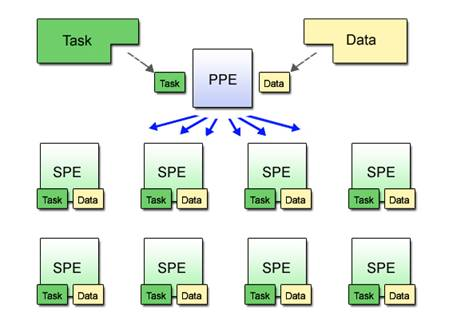
\includegraphics[width=.4\textwidth]{images/cell.jpg}
\end{center}
\hfill (from the Linux Cell documentation)

CUDA (Compute Unified Device Architecture) is NVIDIA's architecture
for processing on GPUs. ``C for CUDA'' predates OpenCL; NVIDIA still
makes CUDA tools available, and they may be faster than OpenCL on NVIDIA
hardware. On recent devices, you can use (most) C++ features in CUDA code,
which you can't do in OpenCL code. We used to do this in OpenCL, but it seems
to be the case that CUDA has got widespread acceptance out in industry, so we
have chosen to use CUDA in the course. If you really need cross-platform or 
you have AMD hardware, then you want OpenCL. The principles are similar 
enough that you can take what you learned in one toolchain and apply it 
to the other.

\paragraph{Programming Model.} The programming
model for all of these architectures is similar: write the code for
the massively parallel computation (kernel) separately from the main
code, transfer the data to the GPU coprocessor (or execute it on the
CPU), wait, then transfer the results back.

OpenCL includes both task parallelism and data parallelism, as we've
discussed earlier in this course. \emph{Data parallelism} is central to
OpenCL; in OpenCL's view, you are evaluating a function, or \emph{kernel},
at a set of points, like so:

\begin{center}

\begin{tikzpicture}
\foreach \x in {0,0.25,...,2}
  \foreach \y in {0,0.25,...,2}
    \draw (\x, \y) circle (0.25mm);
\end{tikzpicture}
\end{center}

Another name for the set of points is the \emph{index space}. 
Each of the points corresponds to a \emph{work-item}.

OpenCL also supports \emph{task parallelism}: it can run different
kernels in parallel. Such kernels may have a one-point index space.
The documentation doesn't say much about task parallelism.

\paragraph{More on work-items.} The work-item is the fundamental
unit of work in OpenCL. These work-items live on an $n$-dimensional
grid (ND-Range); we've seen a 2-dimensional grid above. You may choose
to divide the ND-Range into smaller work-groups, or the system can
divide the range for you. OpenCL spawns a thread for each work item,
with a unique thread ID. The system runs each work-group on a set of
cores; NVIDIA calls that set a \emph{warp}, while ATI calls it a
\emph{wavefront}. The scheduler assigns work-items to the
warps/wavefronts until there are no more work items left.

\paragraph{Shared memory.} OpenCL makes lots of different types of
memory available to you:

\begin{itemize}
\item private memory: available to a single work-item;
\item local memory (aka ``shared memory''): shared between work-items
  belonging to the same work-group; like a user-managed cache;
\item global memory: shared between all work-items as well as the host;
\item constant memory: resides on the GPU, and cached. Does not change.
\end{itemize}

There is also host memory, which generally contains the application's
data.

\paragraph{An example kernel.} Let's continue by looking at 
a sample kernel, first written traditionally and then written
as an OpenCL kernel~\cite{khronos}.

{\scriptsize \hspace*{2em} \begin{minipage}{.8\textwidth} \begin{lstlisting}verbatim
  void traditional_mul(int n, const float *a, const float *b, float *c) {
    int i;
    for (i = 0; i < n; i++) c[i] = a[i] * b[i];
  }
    \end{lstlisting}
  \end{minipage}
  }

The same code looks like this as a kernel:

{\scriptsize \hspace*{1em} \begin{minipage}{.8\textwidth} \begin{lstlisting}verbatim
  kernel void opencl_mul(global const float *a, global const float *b, global float *c) {
    int id = get_global_id(0);  // dimension 0
    c[id] = a[id] * b[id];
  }
    \end{lstlisting}
  \end{minipage}
}

You can write kernels in a variant of C. OpenCL takes away some features,
like function pointers, recursion, variable-length arrays, bit fields,
and standard headers; and adds work-items, workgroups, vectors,
synchronization, and declarations of memory type. OpenCL also provides
a library for kernels to use.

\paragraph{Branches.} OpenCL implements a SIMT architecture.
What this means is that the computation for each work-item can branch
arbitrarily. The hardware will execute all branches that any thread in
a warp executed (which can be slow). 

{\scriptsize \hspace*{2em} \begin{minipage}{.5\textwidth}
    \begin{lstlisting}
kernel void contains_branch(global float *a, global float *b) {
    int id = get_global_id(0);
    if (cond) {
        a[id] += 5.0;
    } else {
        b[id] += 5.0;
    }
}
    \end{lstlisting}
      \end{minipage}}

In the above example, the {\tt if} statement will cause
each thread to execute both branches of the {\tt if}, keeping only the
result of the appropriate branch.

Similarly, executing a loop will cause the
workgroup to wait for the maximum number of iterations of the loop in
any work-item.

{\scriptsize \hspace*{2em} \begin{minipage}{.5\textwidth}
    \begin{lstlisting}verbatim
kernel void contains_loop(global float *a, 
                          global float *b) {
    int id = get_global_id(0);
    
    for (i = 0; i < id; i++) {
        b[i] += a[i];
    }
}
    \end{lstlisting}
\end{minipage} }

If you're setting up workgroups, though, you can arrange for all
of the work-items in a workgroup to execute the same branches.

\paragraph{Synchronization.} You might define
workgroups because you can only put barriers and memory fences between
work items in the same workgroup. Different workgroups execute
independently.

OpenCL also supports all of the notions that we've talked about
before: memory fences (read and write), barriers, and the volatile
keyword.  The barrier ({\tt barrier()}) ensures that all of the
threads in the workgroup all reach the barrier before they continue.
Recall that the fence ensures that no load or store instructions
(depending on the type of fence) migrate to the other side of the fence.

\section*{Complete OpenCL Example}
{
\begin{lstlisting}verbatim
// Note by PL: don't use this example as a template; it uses the C bindings!
// Instead, use the C++ bindings as in the other example.
// source: pages 1-9 through 1-11, http://developer.amd.com/wordpress/media/2013/07/AMD_Accelerated_Parallel_Processing_OpenCL_Programming_Guide-rev-2.7.pdf

//
// Copyright (c) 2010 Advanced Micro Devices, Inc. All rights reserved.
//
// A minimalist OpenCL program.
#include <CL/cl.h>
#include <stdio.h>
#define NWITEMS 512

// A simple memset kernel
const char *source =
"__kernel void memset( __global uint *dst )                             \n"
"{                                                                      \n"
"   dst[get_global_id(0)] = get_global_id(0);                           \n"
"}                                                                      \n";

int main(int argc, char ** argv)
{
   // 1. Get a platform.
   cl_platform_id platform;
   clGetPlatformIDs( 1, &platform, NULL );

   // 2. Find a gpu device.
   cl_device_id device;
   clGetDeviceIDs( platform, CL_DEVICE_TYPE_GPU,
		   1,
		   &device,
		   NULL);

   // 3. Create a context and command queue on that device.
   cl_context context = clCreateContext( NULL,
					 1,
					 &device,
					 NULL, NULL, NULL);
   cl_command_queue queue = clCreateCommandQueue( context,
						  device,
						  0, NULL );
   // 4. Perform runtime source compilation, and obtain kernel entry point.
   cl_program program = clCreateProgramWithSource( context,
						   1,
						   &source,
						   NULL, NULL );
   clBuildProgram( program, 1, &device, NULL, NULL, NULL );
   cl_kernel kernel = clCreateKernel( program, "memset", NULL );
   // 5. Create a data buffer.
   cl_mem buffer = clCreateBuffer( context,
				   CL_MEM_WRITE_ONLY,
				   NWITEMS * sizeof(cl_uint),
				   NULL, NULL );
   // 6. Launch the kernel. Let OpenCL pick the local work size.
   size_t global_work_size = NWITEMS;
   clSetKernelArg(kernel, 0, sizeof(buffer), (void*) &buffer);
   clEnqueueNDRangeKernel( queue,
			   kernel,
			   1,       // dimensions
			   NULL,    // initial offsets
			   &global_work_size, // number of work-items
			   NULL,    // work-items per work-group
                           0, NULL, NULL);  // events
   clFinish( queue );
   // 7. Look at the results via synchronous buffer map.
   cl_uint *ptr;
   ptr = (cl_uint *) clEnqueueMapBuffer( queue,
					 buffer,
					 CL_TRUE,
					 CL_MAP_READ,
					 0,
					 NWITEMS * sizeof(cl_uint),
					 0, NULL, NULL, NULL );
   int i;
   for(i=0; i < NWITEMS; i++)
       printf("%d %d\n", i, ptr[i]);
   return 0;
}
\end{lstlisting}
}

\paragraph{Walk-through.} Let's look at all of the code in the example and
explain the terms. 1) First, we request an OpenCL \emph{platform}.
Platforms, also known as hosts, contain 2) OpenCL \emph{compute devices},
which may in turn contain multiple compute units. Note that we could
also request a CPU device in step 2, without changing the rest of the code.

Next, in step 3, we request an OpenCL \emph{context} (representing all
OpenCL state) and create a \emph{command-queue}. We will request that
OpenCL do work by telling it to run a kernel in the queue.

In step 4, we create an OpenCL \emph{program}. This is a confusing
term; an OpenCL program is what runs on the compute unit, and includes
kernels, functions, and declarations. Your application can contain
more than one OpenCL program. In this case, we create a program
from the C string {\tt source}, which contains the kernel
{\tt memset}. OpenCL can also create programs from binaries, which may be
in an intermediate representation, or already compiled for a particular
device. We get a pointer to the kernel in this step, as the return
value from {\tt clCreateKernel}.

There's one more step before launching the kernel; in step 5, we
create a \emph{data buffer}, which enables communication between
devices. Recall that OpenCL requires explicit communication,
which we'll see later. Since this example doesn't have input, we 
don't need to put anything into the buffer initially.

Finally, we can launch the kernel in step 6. In this case, we don't
specify anything about workgroups, but enqueue the entire
1-dimensional index space, starting at $(0)$. We also state that the
index space has {\tt NWITEMS} elements, and not to subdivide the
problem into work-items. The last three parameters are about events.
We call {\tt clFinish()} to wait for the command-queue to empty.

Finally, in step 7, we copy the results back from the shared buffer
using {\tt clEnqueueMapBuffer}. This copy is blocking (first {\tt
  CL\_TRUE} argument), so we don't need an explicit {\tt clFinish()}
call. We also indicate the details of the command we'd like to
run: in particular, a read of {\tt NWITEMS} from the buffer.

You might also want to consider cleaning up the objects you've
allocated; I haven't shown that here. The code also doesn't contain
any error-handling.

It's important to note that this is a large amount of setup and accordingly overhead cost. Doing the setup, copying the data in, waiting, and copying the data out, all take time. But the GPU can do lots of work in parallel once it gets going. This is a lot like deciding whether to drive or fly. 

If the distance is short, say, 200 km (the distance between Ottawa and Montreal) then flying makes no sense: you have to get to the airport, be there at least an hour or two early to make your way through security checkpoints, then fly, then get from the destination airport to your final destination. Sure, the flying part is fast, but the overhead makes your total average speed not worth it.

On the other hand, if you're going a longer distance, like 4000 km (roughly the distance between Waterloo and San Francisco), then driving is way slower! Sure, the overhead of going the airport remains, but once you're in the air you're moving at 800 km/h or so and in 5.5 hours you are there. Compare that to 40 hours of driving.

\paragraph{C++ Bindings.}
    If we use the C++ bindings, we'll get automatic resource release and
      exceptions.
 C++ likes to use the RAII style
          (resource allocation is initialization).

\begin{itemize}
\item    Change the header to {\tt CL/cl.hpp} and define
      {\tt \_\_CL\_ENABLE\_EXCEPTIONS}.
\end{itemize}

We'd also like to store our kernel in a file instead of a string.
The C API is not so nice to work with; the C++ API is nicer. Use it!
As an example, you'll find the {\tt vector\_add} example in the slides and
in the code repo. 


\section*{More Complicated Kernel}
I've omitted the C code. it's pretty similar to what we saw
before, but it uses workgroups, customized to the number of
compute units on the device.  Here is a more interesting kernel, also from the same source.

{
\begin{lstlisting}verbatim
#pragma OPENCL EXTENSION cl_khr_local_int32_extended_atomics : enable
#pragma OPENCL EXTENSION cl_khr_global_int32_extended_atomics : enable
                                                                    
// 9. The source buffer is accessed as 4-vectors.                  
__kernel void minp( __global uint4 *src,                            
                    __global uint  *gmin,
                    __local uint   *lmin,                             
                    __global uint  *dbg,                             
                    size_t          nitems,                          
                    uint            dev )                            
{                                                                   
  // 10. Set up __global memory access pattern.                    
  uint count  = ( nitems / 4 ) / get_global_size(0);                
  uint idx    = (dev == 0) ? get_global_id(0) * count             
                           : get_global_id(0);                    
  uint stride = (dev == 0) ? 1 : get_global_size(0);               
  uint pmin   = (uint) -1;                                        
                                                                    
  // 11. First, compute private min, for this work-item.           
  for( int n=0; n < count; n++, idx += stride )                    
  {                                                                
    pmin = min( pmin, src[idx].x );                               
    pmin = min( pmin, src[idx].y );                               
    pmin = min( pmin, src[idx].z );                               
    pmin = min( pmin, src[idx].w );                               
  }                                                                
                                                                    
  // 12. Reduce min values inside work-group.                      
  if( get_local_id(0) == 0 )                                       
    lmin[0] = (uint) -1;                                          
  barrier( CLK_LOCAL_MEM_FENCE );                                  

  (void) atom_min( lmin, pmin );                                   
  barrier( CLK_LOCAL_MEM_FENCE );                                  
                                                                    
  // Write out to __global.                                        
  if( get_local_id(0) == 0 )                                       
    gmin[ get_group_id(0) ] = lmin[0];                            
                                                               
  // Dump some debug information.                             
  if( get_global_id(0) == 0 )
     { dbg[0] = get_num_groups(0); dbg[1] = get_global_size(0); 
       dbg[2] = count; dbg[3] = stride; }
}
                                                               
// 13. Reduce work-group min values from __global to __global. 
__kernel void reduce( __global uint4 *src, __global uint *gmin )                    
{                                                              
   (void) atom_min( gmin, gmin[get_global_id(0)] ) ;           
}                                                              
\end{lstlisting}
}

Let's discuss the notable features of this code, which finds the
minimum value from an array of 32-bit ints. (OpenCL ints are always 32
bits). Steps 1 through 8 are in the C code, which I've omitted; see
the AMD guide for the code. At 9), we can investigate the signature of
the {\tt minp} kernel. The use of {\tt uint4}, or 4-int vectors,
enables SSE instructions on CPUs and helps out GPUs as well. We'll
access the constituent {\tt int}s of {\tt src} using the {\tt .x},
{\tt .y}, {\tt .z} and {\tt .w} fields.  This kernel also writes to an
array of global minima, {\tt gmin}, and an array of local minima
(inside the workgroup), {\tt lmin}.

In step 10, we figure out where our point in the index space, as
reported by {\tt get\_global\_id()}, is located in the {\tt src}
index, as well as the stride, which is 1 for CPUs and $7 \times 64
\times c$, where $c$ is the number of work units, which was rounded up
using the following heuristic:

{
\begin{lstlisting}verbatim
  cl_uint ws = 64;
  global_work_size = compute_units * 7 * ws; // 7 wavefronts per SIMD
  while ( (num_src_items / 4) % global_work_size != 0 )
    global_work_size += ws;

  local_work_size = ws;
\end{lstlisting}
}


The core of the kernel occurs in step 11, where the {\tt for}-loop
computes the local minimum of the array elements in the work-item.  In
this stage, we are reading from the {\tt \_\_global} array {\tt src},
and writing to the private memory {\tt pmin}. This takes almost all of
the bandwidth. 

Then, in stage 12, thread 0 of the workgroup initializes the
workgroup-local {\tt lmin} value, and each thread atomically compares
(using the extended atomic requested using the pragma) its {\tt pmin}
to the local {\tt lmin} value.  We have local memory fences here to
make sure that threads stay in synch.  This code is not going to
consume much memory bandwidth, since there aren't many threads per
work-group, and there's only local communication.

Finally, thread 0 of the workgroup writes the local minimum of the
workgroup to the global array {\tt gmin}. In step 13, a second kernel
traverses the {\tt gmin} array and finds the smallest minimum.

\paragraph{Summary.} We've now seen the basics of GPU programming.
The key idea is to define a kernel and find a suitable index space.
Then you execute the kernel over the index space and collect results.
The main difficulty is in formulating your problem in such a way that
you can parallelize it, and then in splitting it into workgroups.


\section*{C++ Bindings Example}
Use the C++ bindings. They're better.

\begin{lstlisting}
// Vector add example, C++ bindings (use these!)
// source:
//  http://www.thebigblob.com/getting-started-
//        with-opencl-and-gpu-computing/

#define __CL_ENABLE_EXCEPTIONS

#include <CL/cl.hpp>

#include <iostream>
#include <fstream>
#include <string>
#include <utility>
#include <vector>
 
int main() {
    // Create the two input vectors
    const int LIST_SIZE = 1000;
    int *A = new int[LIST_SIZE]; 
    int *B = new int[LIST_SIZE];
    for(int i = 0; i < LIST_SIZE; i++) {
        A[i] = i;
        B[i] = LIST_SIZE - i;
    }

    try { 
        // Get available platforms
        std::vector<cl::Platform> platforms;
        cl::Platform::get(&platforms);

        // Select the default platform and create a context
        // using this platform and the GPU
        cl_context_properties cps[3] = { 
            CL_CONTEXT_PLATFORM, 
            (cl_context_properties)(platforms[0])(), 
            0 
        };
        cl::Context context(CL_DEVICE_TYPE_GPU, cps);
 
        // Get a list of devices on this platform
        std::vector<cl::Device> devices =
            context.getInfo<CL_CONTEXT_DEVICES>();
 
        // Create a command queue and use the first device
        cl::CommandQueue queue = cl::CommandQueue(context,
            devices[0]);

        // Read source file
        std::ifstream sourceFile("vector_add_kernel.cl");
        std::string sourceCode(
            std::istreambuf_iterator<char>(sourceFile),
            (std::istreambuf_iterator<char>())
        );
        cl::Program::Sources source(
            1,
            std::make_pair(sourceCode.c_str(),
                           sourceCode.length()+1)
        );
 
        // Make program of the source code in the context
        cl::Program program = cl::Program(context, source);
 
        // Build program for these specific devices
        program.build(devices);
 
        // Make kernel
        cl::Kernel kernel(program, "vector_add");
        
        // Create memory buffers
        cl::Buffer bufferA = cl::Buffer(
            context,
            CL_MEM_READ_ONLY,
            LIST_SIZE * sizeof(int)
        );
        cl::Buffer bufferB = cl::Buffer(
            context,
            CL_MEM_READ_ONLY,
            LIST_SIZE * sizeof(int)
        );
        cl::Buffer bufferC = cl::Buffer(
            context,
            CL_MEM_WRITE_ONLY,
            LIST_SIZE * sizeof(int)
        );
        
        // Copy lists A and B to the memory buffers
        queue.enqueueWriteBuffer(
            bufferA,
            CL_TRUE,
            0,
            LIST_SIZE * sizeof(int),
            A
        );
        queue.enqueueWriteBuffer(
            bufferB,
            CL_TRUE,
            0,
            LIST_SIZE * sizeof(int),
            B
        );
 
        // Set arguments to kernel
        kernel.setArg(0, bufferA);
        kernel.setArg(1, bufferB);
        kernel.setArg(2, bufferC);

        // Run the kernel on specific ND range
        cl::NDRange global(LIST_SIZE);
        cl::NDRange local(1);
        queue.enqueueNDRangeKernel(
            kernel,
            cl::NullRange,
            global,
            local
        );
 
        // Read buffer C into a local list
        int* C = new int[LIST_SIZE];
        queue.enqueueReadBuffer(
             bufferC,
             CL_TRUE,
             0,
             LIST_SIZE * sizeof(int),
             C
        );

        for(int i = 0; i < LIST_SIZE; i ++) {
            std::cout << A[i] << " + " << B[i] << " = "
                      << C[i] << std::endl;
        }
    } catch(cl::Error error) {
        std::cout << error.what() << "(" << error.err()
                  << ")" << std::endl;
    }
 
    return 0;
}
\end{lstlisting}

\bibliographystyle{alphaurl}
\bibliography{459}


\end{document}
